% !TEX root = ../thesis-example.tex
%
\chapter{Appendix}
\label{sec:appendix}


\section{Figures}
\label{sec:appendix:lrf_imgs}

\subsection{Evaluated Market}
\label{sec:appendix:lrf_imgs:market_evald}
\begin{figure}[ht]
    \centering
	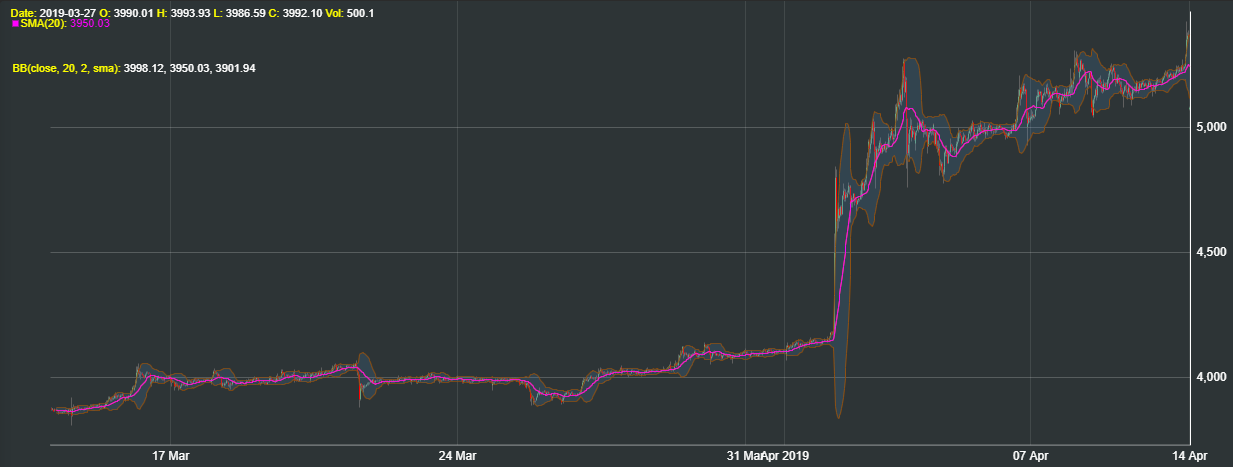
\includegraphics[angle=90,width=0.42\textwidth]{content/graphics/market_evaluated.PNG}
	\caption{The \textbf{BTC / USDT }coin pair's candlestick chart from the \textbf{13-03-19} to the \textbf{10-04-19}; The market mostly moves sideways from the start of March until the start of April where a significant increase in price occurs}
	\label{fig:eval:strats:market_evald}
\end{figure}




\section{Code Snippets}
\label{sec:appendix:code_snippets}

\begin{code}
\captionof{listing}{pandas Example 1}
\label{code:rel:dev_lib:pandas:amz_data}
\begin{minted}{Python}
import pandas_datareader.data as web
# collect data for Amazon from 2017-04-22 to 2018-04-22
start = '2017-04-22'
end = '2018-04-22'
df = web.DataReader(name='AMZN', data_source='iex', start=start, end=end)
print(df)
\end{minted}
\begin{minted}{text}
// OUTPUT
open date    high      low        close      volume
2017-04-24   908.680   909.9900   903.8200   907.41   3122893
2017-04-25   907.040   909.4800   903.0000   907.62   3380639
...
\end{minted}
\end{code}

\begin{code}
\captionof{listing}{Backtrader Differences Between Moving Averages}
\label{code:rel:dev_lib:backtrader:sma_diff}
\begin{minted}{Python}
a = SMA(period=25) - SMA(period=50)
\end{minted}
\end{code}


\begin{code}
\captionof{listing}{Flask RESTful Minimal Setup}
\label{code:rel:dev_lib:flask:flask_restful}
\begin{minted}{Python}
from flask import Flask
from flask_restful import Resource, Api

app = Flask(__name__)
api = Api(app)

class HelloWorld(Resource):
    def get(self):
        return {'hello': 'world'}

api.add_resource(HelloWorld, '/')

if __name__ == '__main__':
    app.run(debug=True)
\end{minted}
\end{code}


\begin{code}
\captionof{listing}{Calculating When The Next API Call Is Allowed}
\label{code:impl:exchange_data:calc_next_interval}
\begin{minted}{Python}
# msOccuredAt is the time a 429 code is received
# Calculation is done in millieseconds, e.g. 60000ms = 1 minute
nextCallAt = floor( ( msOccuredAt / 60000) + 1) * 60000
\end{minted}
\end{code}


\newpage
\section{Use cases}

\subsection{Non-Functional Use cases}
\label{sec:requirements:non_func:usecases}
%Sometimes it is a good idea to put domain objects in \texttt{}
%The template and the descriptions are based on the book Applying UML and Patterns: 
%An Introduction to Object-Oriented Analysis and Design and Iterative Development
%(3rd Edition) by Craig Larman.
\begin{usecase}

\addtitle{Use Case 1}{API Data Retrieval} 
\label{sec:requirements:non_func:usecases:1}

%Scope: the system under design
\addfield{Scope:}{Binance Communication Monitor}

%Level: "user-goal" or "subfunction"
\addfield{Level:}{subfunction}

%Primary Actor: Calls on the system to deliver its services.
\addfield{Primary Actor:}{Connection Monitor}

%Stakeholders and Interests: Who cares about this use case and what do they want?
\additemizedfield{Stakeholders and \\ Interests:}{
	\item Developers: Ensures bot can access data
	\item Users: Ensures bot can generate trade signals
}

%Preconditions: What must be true on start and worth telling the reader?
\addfield{Preconditions:}{Requirement of data}
%when multiple
%\additemizedfield{Preconditions:}{} 

%Postconditions: What must be true on successful completion and worth telling the reader
\addfield{Postconditions:}{Retrevial of data}
%when multiple
%\additemizedfield{Preconditions:}{}

%Main Success Scenario: A typical, unconditional happy path scenario of success.
\addscenario{Main Success Scenario:}{
	\item The bot requires data from Binance API
	\item Fetch request is sent for data
	\item Data returns without warnings
}

%Extensions: Alternate scenarios of success or failure.
\addscenario{Extensions:}{
	\item[3.a] Warning code \textbf{429} is returned:
	    \begin{enumerate}
    	\item[1.] Weight Tracker sets a delay to prevent further spamming
    	\item[2.] Delay time passes
    	\item[3.] Continue fetching data as usual
    	\item[4.] Alternative use case ends
	    \end{enumerate}
	\item[3.b.] Warning code \textbf{429} is returned:
		\begin{enumerate}
    	\item[1.] Attempt to fetch data as usual
		\item[2.] Warning code \textbf{418} returned (IP Banned)
		\item[3.] Bot logs IP ban and warns user
		\item[4.] Alternative use case ends
		\end{enumerate}
}

%Special Requirements: Related non-functional requirements.
\additemizedfield{Special \\ Requirements:}{
	\item NFR-1 at table \ref{table:requirements:non_func}
	\item NFR-2 at table \ref{table:requirements:non_func}
}

%Technology and Data Variations List: Varying I/O methods and data formats.
\addscenario{Technology and Data Variations List:}{
	\item[2.a.] Opens web socket connection
	    \begin{enumerate}
    	\item[1.] Receives data by push update at 1 second intervals
    	\item[2.] Alternative use case ends
	    \end{enumerate}
}

%Frequency of Occurrence: Influences investigation, testing and timing of implementation.
%\addfield{Frequency of Occurrence:}{}

%Miscellaneous: Such as open issues/questions
%\addfield{Open Issues:}{}

\end{usecase}


\begin{usecase}

\addtitle{Use Case 2}{Perform Trade Process} 
\label{sec:requirements:non_func:usecases:2}

%Scope: the system under design
\addfield{Scope:}{Trade Process}

%Level: "user-goal" or "subfunction"
\addfield{Level:}{subfunction}

%Primary Actor: Calls on the system to deliver its services.
\addfield{Primary Actor:}{Technical Analysis Calculator}

%Stakeholders and Interests: Who cares about this use case and what do they want?
\additemizedfield{Stakeholders and \\ Interests:}{
    \item Developer: No backlog of data
	\item User: Up-to-date technical analysis 
}

%Preconditions: What must be true on start and worth telling the reader?
\additemizedfield{Preconditions:}{
    \item Historical data has been retrieved and evaluated
    \item Real-time data is currently being push to function
}
%when multiple
%\additemizedfield{Preconditions:}{} 

%Postconditions: What must be true on successful completion and worth telling the reader
\addfield{Postconditions:}{Technical analysis of real-time data before next day is pushed}
%when multiple
%\additemizedfield{Preconditions:}{}

%Main Success Scenario: A typical, unconditional happy path scenario of success.
\addscenario{Main Success Scenario:}{
	\item Perform technical analysis on push data
	\item Finish evaluation and push outcome
	\item Waits for new data
}

%Extensions: Alternate scenarios of success or failure.
\addscenario{Extensions:}{
	\item[2.a.] New data is pushed while still evaluating:
	    \begin{enumerate}
    	\item[1.] Finish evaluation and push outcome
    	\item[2.] Repeat from step 1
    	\item[3.] Data is continually pushed
    	\item[4.] Queue reaches threshold
    	\item[5.] Bot cancels operations, logs errors and performs shutdown
    	\item[6.] Alternative use case ends
	    \end{enumerate}
}

%Special Requirements: Related non-functional requirements.
\additemizedfield{Special \\ Requirements:}{
	\item NFR-3 at table \ref{table:requirements:non_func}
}

%Technology and Data Variations List: Varying I/O methods and data formats.
%\addscenario{Technology and Data Variations List:}{}

%Frequency of Occurrence: Influences investigation, testing and timing of implementation.
%\addfield{Frequency of Occurrence:}{}

%Miscellaneous: Such as open issues/questions
%\addfield{Open Issues:}{}

\end{usecase}



\begin{usecase}

\addtitle{Use Case 3}{Trade Execution} 
\label{sec:requirements:non_func:usecases:3}

%Scope: the system under design
\addfield{Scope:}{Trade Execution}

%Level: "user-goal" or "subfunction"
\addfield{Level:}{subfunction}

%Primary Actor: Calls on the system to deliver its services.
\addfield{Primary Actor:}{Trade Executor}

%Stakeholders and Interests: Who cares about this use case and what do they want?
\additemizedfield{Stakeholders and \\ Interests:}{
    \item Developer: Enters/Exits Positions Cleanly
	\item User: Minimise Transaction Costs 
}

%Preconditions: What must be true on start and worth telling the reader?
\additemizedfield{Preconditions:}{
    \item Trade Signal Received
    \item Fetched Real-time Order Book Depth Data 
}
%when multiple
%\additemizedfield{Preconditions:}{} 

%Postconditions: What must be true on successful completion and worth telling the reader
\addfield{Postconditions:}{Trade Executed Fully}
%when multiple
%\additemizedfield{Preconditions:}{}

%Main Success Scenario: A typical, unconditional happy path scenario of success.
\addscenario{Main Success Scenario:}{
    \item Apply user settings to trade
	\item Evaluate depth data 
	\item Find enter/exit price
	\item Determine order type
	\item Send trade details to execute
	\item Receive acknowledgement
	\item Monitor order status
	\item Update portfolio data on success 
}

%Extensions: Alternate scenarios of success or failure.
\addscenario{Extensions:}{
	\item[8.a.] Order fails to fill:
	    \begin{enumerate}
    	\item[1.] Back trace to step 2
    	\item[2.] Evaluate data is still suitable from user settings
    	\item[3.] Confirmation market fits into users settings
    	\item[4.] Back trace to step 3
    	\item[5.] Alternative use case ends
	    \end{enumerate}
	\item[8.b.] Start at 8.a.3:
	    \begin{enumerate}
	        \item[1.]  Determine market doesn't fit into users settings
    	    \item[2.] Return back to trade signal generation
    	    \item[3.] Alternative use case ends
	    \end{enumerate}
}

%Special Requirements: Related non-functional requirements.
\additemizedfield{Special \\ Requirements:}{
	\item NFR-4 at table \ref{table:requirements:non_func}
	\item FR-5 at table \ref{table:requirements:func}
}

%Technology and Data Variations List: Varying I/O methods and data formats.
%\addscenario{Technology and Data Variations List:}{}

%Frequency of Occurrence: Influences investigation, testing and timing of implementation.
%\addfield{Frequency of Occurrence:}{}

%Miscellaneous: Such as open issues/questions
%\addfield{Open Issues:}{}

\end{usecase}


\subsection{Functional Use cases}
\label{sec:requirements:func:usecases}


\begin{usecase}

\addtitle{Use Case 1}{Start Bot Operation} 
\label{sec:requirements:func:usecases:1}

%Scope: the system under design
\addfield{Scope:}{Start Bot}

%Level: "user-goal" or "subfunction"
\addfield{Level:}{user-goal}

%Primary Actor: Calls on the system to deliver its services.
\addfield{Primary Actor:}{User}

%Stakeholders and Interests: Who cares about this use case and what do they want?
\additemizedfield{Stakeholders and \\ Interests:}{
	\item Developers: Ensures bot can deliver operations
	\item Users: Use the bot to automate trades
}

%Preconditions: What must be true on start and worth telling the reader?
\addfield{Preconditions:}{
    Active Internet Connection
}
%when multiple
%\additemizedfield{Preconditions:}{} 

%Postconditions: What must be true on successful completion and worth telling the reader
\addfield{Postconditions:}{Technical analysis on selected coin}
%when multiple
%\additemizedfield{Preconditions:}{}

%Main Success Scenario: A typical, unconditional happy path scenario of success.
\addscenario{Main Success Scenario:}{
    \item User selects coin and configures algorithm options
	\item User sends start signal and configuration to server
	\item Bot analyses and fetches data required
	\item Bot performs technical analysis repeatedly
	\item Bot generates trade signal when indicators align
	\item Bot alerts user
	\item Bot sends trade details to Binance
	\item Bot updates user details on success
	\item Bot alerts user
}

%Extensions: Alternate scenarios of success or failure.
\addscenario{Extensions:}{
	\item[4.a] Bot warns user of risky coin choice:
	    \begin{enumerate}
	    \item[1.] User confirms warning
    	\item[2.] Back trace to step 4
    	\item[3.] Alternative use case ends
	    \end{enumerate}
	\item[4.b.] Start from 4.a:
		\begin{enumerate}
		\item[1.] Try counter is greater than threshold
    	\item[2.] Log error
		\item[3.] Alert user unable to cancel active orders
		\item[4.] Back trace to step 5
		\item[5.] Alternative use case ends
		\end{enumerate}
}

%Special Requirements: Related non-functional requirements.
\additemizedfield{Special \\ Requirements:}{
	\item NFR-8 at table \ref{table:requirements:non_func}
	\item FR-1 at table \ref{table:requirements:func}
	\item FR-2 at table \ref{table:requirements:func}
}

%Technology and Data Variations List: Varying I/O methods and data formats.
%\addscenario{Technology and Data Variations List:}{}

%Frequency of Occurrence: Influences investigation, testing and timing of implementation.
%\addfield{Frequency of Occurrence:}{}

%Miscellaneous: Such as open issues/questions
%\addfield{Open Issues:}{}

\end{usecase}



\begin{usecase}

\addtitle{Use Case 2}{Stop Bot Operation} 
\label{sec:requirements:func:usecases:2}
%Scope: the system under design
\addfield{Scope:}{Stop Bot}

%Level: "user-goal" or "subfunction"
\addfield{Level:}{user-goal}

%Primary Actor: Calls on the system to deliver its services.
\addfield{Primary Actor:}{User}

%Stakeholders and Interests: Who cares about this use case and what do they want?
\additemizedfield{Stakeholders and \\ Interests:}{
	\item Developers: Ensures user has control over the bots operations
	\item Users: Control over the bots operation
}

%Preconditions: What must be true on start and worth telling the reader?
\addfield{Preconditions:}{
    Active Internet Connection
}
%when multiple
%\additemizedfield{Preconditions:}{} 

%Postconditions: What must be true on successful completion and worth telling the reader
\addfield{Postconditions:}{All technical analysis and pending trades are cancelled}
%when multiple
%\additemizedfield{Preconditions:}{}

%Main Success Scenario: A typical, unconditional happy path scenario of success.
\addscenario{Main Success Scenario:}{
	\item User sends a stop signal to the server
	\item Server begins stop procedure for bot
	\item Request is sent to Binance API to cancel all orders
	\item Receive acknowledgement
	\item Close web sockets and prevent further communication
	\item Stop trade signal generation
	\item Bot displays confirmation message to user
}

%Extensions: Alternate scenarios of success or failure.
\addscenario{Extensions:}{
	\item[4.a] Incorrect acknowledgement code:
	    \begin{enumerate}
	    \item[1.] Try counter is less than threshold
    	\item[2.] Increment counter
    	\item[3.] Back trace to step 3
    	\item[4.] Alternative use case ends
	    \end{enumerate}
	\item[4.b.] Start from 4.a:
		\begin{enumerate}
		\item[1.] Try counter is greater than threshold
    	\item[2.] Log error
		\item[3.] Alert user unable to cancel active orders
		\item[4.] Back trace to step 5
		\item[5.] Alternative use case ends
		\end{enumerate}
}

%Special Requirements: Related non-functional requirements.
\additemizedfield{Special \\ Requirements:}{
	\item NFR-8 at table \ref{table:requirements:non_func}
	\item FR-1 at table \ref{table:requirements:func}
	\item FR-2 at table \ref{table:requirements:func}
}

%Technology and Data Variations List: Varying I/O methods and data formats.
%\addscenario{Technology and Data Variations List:}{}

%Frequency of Occurrence: Influences investigation, testing and timing of implementation.
%\addfield{Frequency of Occurrence:}{}

%Miscellaneous: Such as open issues/questions
%\addfield{Open Issues:}{}

\end{usecase}



\begin{usecase}

\addtitle{Use Case 3}{Display Chart Information} 
\label{sec:requirements:func:usecases:3}
%Scope: the system under design
\addfield{Scope:}{Chart User Interface}

%Level: "user-goal" or "subfunction"
\addfield{Level:}{subfunction}

%Primary Actor: Calls on the system to deliver its services.
\addfield{Primary Actor:}{Server}

%Stakeholders and Interests: Who cares about this use case and what do they want?
\additemizedfield{Stakeholders and \\ Interests:}{
	\item Developers: Ensures data can be displayed in an intuitive way
	\item Users: Understand the market from visual cue
}

%Preconditions: What must be true on start and worth telling the reader?
\addfield{Preconditions:}{
    Active Internet Connection
}
%when multiple
%\additemizedfield{Preconditions:}{} 

%Postconditions: What must be true on successful completion and worth telling the reader
\addfield{Postconditions:}{Candlestick Chart Displays Real-Time Data}
%when multiple
%\additemizedfield{Preconditions:}{}

%Main Success Scenario: A typical, unconditional happy path scenario of success.
\addscenario{Main Success Scenario:}{
    \item User opens trade bot URL
    \item Automatic request to server for data
    \item Server gathers data locally
    \item Server adds User to web socket push data
    \item Server sends data to front end
    \item Front end parses data to chart
}

%Extensions: Alternate scenarios of success or failure.
\addscenario{Extensions:}{
	\item[3.a] No up-to-date local data for coin:
	    \begin{enumerate}
	    \item[1.] Server retrieves data from Binance API
    	\item[2.] Stores data locally for future use
    	\item[3.] Continue to step 4
    	\item[4.] Alternative use case ends
	    \end{enumerate}
}

%Special Requirements: Related non-functional requirements.
\additemizedfield{Special \\ Requirements:}{
    \item NFR-6 at table \ref{table:requirements:non_func}
	\item NFR-8 at table \ref{table:requirements:non_func}
	\item FR-3 at table \ref{table:requirements:func}
	\item FR-2 at table \ref{table:requirements:func}
}

%Technology and Data Variations List: Varying I/O methods and data formats.
%\addscenario{Technology and Data Variations List:}{}

%Frequency of Occurrence: Influences investigation, testing and timing of implementation.
%\addfield{Frequency of Occurrence:}{}

%Miscellaneous: Such as open issues/questions
%\addfield{Open Issues:}{}

\end{usecase}



\begin{usecase}

\addtitle{Use Case 4}{Display Back-Testing Results} 
\label{sec:requirements:func:usecases:4}
%Scope: the system under design
\addfield{Scope:}{Chart User Interface}

%Level: "user-goal" or "subfunction"
\addfield{Level:}{User-goal}

%Primary Actor: Calls on the system to deliver its services.
\addfield{Primary Actor:}{User}

%Stakeholders and Interests: Who cares about this use case and what do they want?
\additemizedfield{Stakeholders and \\ Interests:}{
	\item Developers: Ensures algorithms can be tested on historical data
	\item Users: Analyse the algorithms performance on historical data
}

%Preconditions: What must be true on start and worth telling the reader?
\additemizedfield{Preconditions:}{
    \item Active Internet Connection
    \item Historical Market Data for Coin
    
}
%when multiple
%\additemizedfield{Preconditions:}{} 

%Postconditions: What must be true on successful completion and worth telling the reader
\addfield{Postconditions:}{Candlestick Chart Displays Historical Trade Signals}
%when multiple
%\additemizedfield{Preconditions:}{}

%Main Success Scenario: A typical, unconditional happy path scenario of success.
\addscenario{Main Success Scenario:}{
    \item User specifies options
    \item User requests back-testing results
    \item Server applies criteria 
    \item Server applies data
    \item Server sends results to front end chart
}


%Extensions: Alternate scenarios of success or failure.
\addscenario{Extensions:}{
	\item[6.] Reset to default display:
	    \begin{enumerate}
	    \item[1.] User signals front end to reset chart
    	\item[2.] Front end chart removes added indicators
    	\item[3.] Alternative use case ends
	    \end{enumerate}
}

%Special Requirements: Related non-functional requirements.
\additemizedfield{Special \\ Requirements:}{
	\item NFR-8 at table \ref{table:requirements:non_func}
	\item FR-5 at table \ref{table:requirements:func}
	\item FR-6 at table \ref{table:requirements:func}
}

%Technology and Data Variations List: Varying I/O methods and data formats.
%\addscenario{Technology and Data Variations List:}{}

%Frequency of Occurrence: Influences investigation, testing and timing of implementation.
%\addfield{Frequency of Occurrence:}{}

%Miscellaneous: Such as open issues/questions
%\addfield{Open Issues:}{}

\end{usecase}



\definecolor{barblue}{RGB}{153,204,254}
\definecolor{groupblue}{RGB}{51,102,254}
\definecolor{linkred}{RGB}{165,0,33}
\renewcommand\sfdefault{phv}
\renewcommand\mddefault{mc}
\renewcommand\bfdefault{bc}
\setganttlinklabel{s-s}{START-TO-START}
\setganttlinklabel{f-s}{FINISH-TO-START}
\setganttlinklabel{f-f}{FINISH-TO-FINISH}
\sffamily



\section{Gantt Charts}
\label{sec:appendix:gantt}

\subsection{Semester 1 Gantt Chart}
\label{gantt:sem1}
   \noindent \begin{ganttchart}[
        canvas/.append style={fill=none, draw=black!5, line width=.75pt},
        hgrid style/.style={draw=black!5, line width=.75pt},
        vgrid={*1{draw=black!5, line width=.75pt}},
        today=11,
        today rule/.style={
          draw=black!64,
          dash pattern=on 3.5pt off 4.5pt,
          line width=1.5pt
        },
        today label font=\small\bfseries,
        title/.style={draw=none, fill=none},
        title label font=\bfseries\footnotesize,
        title label node/.append style={below=7pt},
        include title in canvas=false,
        bar label font=\mdseries\small\color{black!70},
        bar label node/.append style={left=2cm},
        bar/.append style={draw=none, fill=black!63},
        bar incomplete/.append style={fill=barblue},
        bar progress label font=\mdseries\footnotesize\color{black!70},
        group incomplete/.append style={fill=groupblue},
        group left shift=0,
        group right shift=0,
        group height=.5,
        group peaks tip position=0,
        group label node/.append style={left=.6cm},
        group progress label font=\bfseries\small,
        link/.style={-latex, line width=1.5pt, linkred},
        link label font=\scriptsize\bfseries,
        link label node/.append style={below left=-2pt and 0pt}
      ]{1}{13}
      \gantttitle[
        title label node/.append style={below left=7pt and -3pt}
      ]{WEEKS:\quad1}{1}
      \gantttitlelist{2,...,13}{1} \\
      
      \ganttgroup[progress=100]{Deliverable 1}{1}{11} \\
      \ganttbar[
        progress=100,
        name=TASK11
      ]{\textbf{Task 1.1} Supervisor Meeting}{1}{1} \\
      \ganttbar[
        progress=100,
        name=TASK12
      ]{\textbf{Task 1.2} Aims \& Objectives}{1}{2} \\
      
      
      \ganttlink[link type=s-s,
        link label node/.append style=right]{TASK11}{TASK12}
      
      
      \ganttgroup[progress=100]{Literature Review}{3}{7} \\
      \ganttbar[progress=100,
        name=TASK21]{\textbf{Task 2.1} Research \& Draft}{3}{5} \\
      \ganttbar[progress=100,
        name=TASK22]{\textbf{Task 2.2} Evaluate \& Finalise}{6}{7} \\
        
        
    \ganttmilestone[name=LIT]{Literature Review Milestone}{7} \\
        
        
      \ganttlink[
        link type=f-s,
        link label node/.append style=right
      ]{TASK21}{TASK22}
      
    \ganttlink[
        link type=dr,
        link label node/.append style=left
      ]{TASK12}{TASK21}
      \ganttlink[
        link type=dr
      ]{TASK22}{LIT}
      
    
      
      
      
      \ganttgroup[progress=80]{Requirements Analysis}{6}{7} \\
      \ganttbar[progress=100,
        name=TASK31]{\textbf{Task 3.1} Identify Requirements}{6}{6} \\
      \ganttbar[progress=60,
        name=TASK32]{\textbf{Task 3.2} Design Use Cases}{7}{7} \\
        
      \ganttlink[
        link type=f-s,
        link label node/.append style=right
      ]{TASK31}{TASK32}
      
      
      
      \ganttgroup[progress=100]{Design Analysis}{6}{8} \\
      \ganttbar[progress=100,
        name=TASK41]{\textbf{Task 4.1} Identify Technology Stack}{6}{7} \\
      \ganttbar[progress=100,
        name=TASK42]{\textbf{Task 4.2} Discuss}{8}{8} \\
        
        \ganttlink[
        link type=dr,
        link label node/.append style=left
      ]{TASK41}{TASK42}
        
      \ganttlink[
        link type=s-s,
        link label node/.append style=right
      ]{TASK31}{TASK41}
      
      \ganttgroup[progress=90]{Evaluation Strategies}{8}{9} \\
      \ganttbar[progress=90,
        name=TASK51]{\textbf{Task 5.1} Identify \& Discuss}{8}{9} \\
        
        \ganttbar[progress=100,
        name=TASK52]{\textbf{Task 5.2} Submit Ethics}{9}{9} \\
        
       \ganttlink[
        link type=f-f,
        link label node/.append style=left
      ]{TASK51}{TASK52}
        
      
      \ganttgroup[progress=95]{Project Plan}{3}{10} \\
      \ganttbar[progress=100,
        name=TASK61]{\textbf{Task 6.1} Plan Semester 1}{3}{4} \\
      \ganttbar[progress=100,
        name=TASK62]{\textbf{Task 6.2} Plan Semester 2}{9}{9} \\
        
        \ganttbar[progress=90,
            name=TASK63]{\textbf{Task 6.3} Risk Analysis}{9}{9} \\
            
    \ganttbar[progress=100,
            name=TASK64]{\textbf{Task 6.4} PLES Analysis}{10}{10} \\
        
      
      \ganttlink[
        link type=s-s,
        link label node/.append style=left
      ]{TASK62}{TASK63}
      
      \ganttmilestone[name=DEL_1]{Deliverable 1 Milestone}{11} 
      
      
    \end{ganttchart}
    
    
    
    
    
    
    
    
\subsection{Semester 2 Gantt Chart}
\label{gantt:sem2}

       \noindent \begin{ganttchart}[
        canvas/.append style={fill=none, draw=black!5, line width=.75pt},
        hgrid style/.style={draw=black!5, line width=.75pt},
        vgrid={*1{draw=black!5, line width=.75pt}},
        title/.style={draw=none, fill=none},
        title label font=\bfseries\footnotesize,
        title label node/.append style={below=7pt},
        include title in canvas=false,
        bar label font=\mdseries\small\color{black!70},
        bar label node/.append style={left=2cm},
        bar/.append style={draw=none, fill=black!63},
        bar incomplete/.append style={fill=barblue},
        bar progress label font=\mdseries\footnotesize\color{black!70},
        group incomplete/.append style={fill=groupblue},
        group left shift=0,
        group right shift=0,
        group height=.5,
        group peaks tip position=0,
        group label node/.append style={left=.6cm},
        group progress label font=\bfseries\small,
        link/.style={-latex, line width=1.5pt, linkred},
        link label font=\scriptsize\bfseries,
        link label node/.append style={below left=-2pt and 0pt}
      ]{1}{13}
      \gantttitle[
        title label node/.append style={below left=7pt and -3pt}
      ]{WEEKS:\quad1}{1}
      \gantttitlelist{2,...,13}{1} \\
      
      \ganttgroup[progress=0]{Project Development}{1}{10} \\
      \ganttbar[
        progress=0,
        name=TASK11
      ]{\textbf{Task 1.1} Supervisor Meeting}{1}{1} \\
      
      \ganttbar[
        progress=0,
        name=TASK12
      ]{\textbf{Task 1.2} Binance Communication}{1}{1} \\
      
      \ganttbar[
        progress=0,
        name=TASK13
      ]{\textbf{Task 1.3} Trade Process}{2}{3} \\
      
      \ganttbar[
        progress=0,
        name=TASK14
      ]{\textbf{Task 1.4} Server Infrastructure}{4}{5} \\
      
      \ganttbar[
        progress=0,
        name=TASK15
      ]{\textbf{Task 1.5} User Interface}{6}{7} \\
      
      \ganttbar[
        progress=0,
        name=TASK16
      ]{\textbf{Task 1.6} Refine \& Evaluate}{8}{9} \\
      
      \ganttmilestone[name=complete_proj]{Project Build 1.0}{9} \\
      
      
      \ganttlink[link type=s-s,
        link label node/.append style=right]{TASK11}{TASK12}
      
      \ganttlink[link type=f-s,
        link label node/.append style=right]{TASK12}{TASK13}
      \ganttlink[link type=f-s,
        link label node/.append style=right]{TASK13}{TASK14}
      \ganttlink[link type=f-s,
        link label node/.append style=right]{TASK14}{TASK15}
      \ganttlink[link type=f-s,
        link label node/.append style=right]{TASK15}{TASK16}
      
      \ganttlink[link type=dr]{TASK16}{complete_proj}
      
      
      \ganttgroup[progress=0]{Dissertation}{2}{12} \\
      \ganttbar[progress=0,
        name=TASK21]{\textbf{Task 2.1} Work Done}{2}{7} \\
      \ganttbar[progress=0,
        name=TASK22]{\textbf{Task 2.2} Test \& Performance Assessment}{8}{9} \\
        
      \ganttmilestone[name=dis_draft]{Dissertation Draft Milestone}{10} \\
      
      \ganttlink[link type=s-s,
        link label node/.append style=right]{TASK13}{TASK21}
      
      \ganttlink[link type=f-s]{TASK21}{TASK22}
      \ganttlink[link type=dr]{TASK22}{dis_draft}
      
      
      \ganttbar[progress=0,
        name=TASK31]{\textbf{Task 3.1} Improve Dissertation}{11}{12} \\
        
         \ganttlink[link bulge=.8]{dis_draft}{TASK31}
        
      \ganttmilestone[name=dis]{Dissertation Hand-In Milestone}{12} \\
    
    
     \ganttlink[link type=dr]{TASK31}{dis}
    
    
    \ganttbar[progress=0,
        name=TASK41]{\textbf{Task 4.1} Poster Session Prep}{12}{13} \\

        
      \ganttlink[link bulge=.8]{dis}{TASK41}
    
    \ganttmilestone[name=post]{Poster Session Milestone}{13} \\
    
    \ganttlink[link type=dr]{TASK41}{post}
        
      
      
    \end{ganttchart}